\section{Zustands-Regler}
\subsection{State Feadback}

$A_g = A-BK \; , \; B_g = BK_{vf} \; , \; C_g = C $\\
$G(s) = \frac{\underline{Y}(s)}{\underline{U}(s)} = C(sI-A+BK)^{-1}BK_{vf}$\\
$K_{vf} = (C(-A+BK)^{-1}B)^{-1}$

\subsection{Pole Placement}

\begin{tabular}{ll}
	\parbox{8cm}{$det(\lambda I-A+BK) = (\lambda - \lambda_1)...(\lambda - \lambda_n)$} &
	\parbox{3cm}{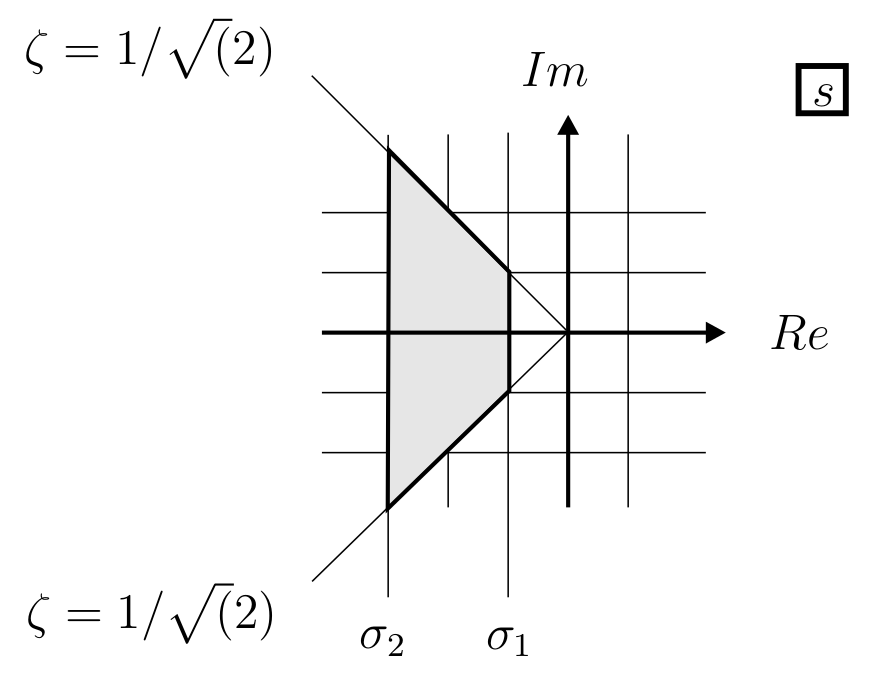
\includegraphics[width=3cm]{./bilder/pole_locations.png}}
\end{tabular}

\newpage

\subsection{LQR-Entwurf (Linear-quadratic regulator)}
	$$J(K_R,T_N,\ldots)=\int\limits^{\infty}_0 e(t)^2 dt = minimal$$\\
	$$J=\int\limits_0^{\infty} {x^T Q x+u^T R u}= minimal$$\\
	Q,R: positive definite; Bei SISO ist R eine Zahl\\
	Optimum: Riccati equation\\
	$ A^T P + P A - P B R^{-1} B^T P = -Q$ \hspace{2cm}
	P ist die L"osungsmatrix
	\begin{aufzaehlung}
    	\item $\dot{x} = Ax + Bu \; / \;  Q \; \text{und} \; R \; \text{gegeben}$
    	\textbf{meist} wird f"ur Q=I und R=1 eingesetzt.
    	\item L"osungsmatrix P bestimmen (aus der L"osungsmenge den positiv
    	definierten Wert)
    	\item Reglervektor berechnen $K=R^{-1} B^T P$
    \end{aufzaehlung}
